\documentclass[11pt]{article}

\usepackage[margin=1in]{geometry}
\usepackage{amsmath,amssymb}
\usepackage{booktabs}
\usepackage{siunitx}
\usepackage{graphicx}
\usepackage[round]{natbib}
\usepackage{hyperref}
\usepackage{xcolor}

\DeclareSIUnit\usd{USD}

\newcommand{\todopending}[1]{{\color{gray!70!black}\itshape[Pending: #1]}}

\title{The Compute Merit Order: Where AI Compute Is Economic to Run}
\author{Compute Merit Order Project}
\date{Working paper --- draft, \today}

\begin{document}
\maketitle

\begin{abstract}
A GPU cluster earns a compute price per GPU-hour and pays an electricity
cost per GPU-hour; the difference is a spread directly analogous to the
spark spread long used in power markets. We propose that this compute
spark spread determines a shutdown price below which a given fleet is
uneconomic to run, and that because industrial electricity costs vary by
roughly a factor of three across regions, shutdown prices should vary
similarly --- implying a predictable global merit order in which capacity
retires by geography as compute prices fall. We further ask whether the
binding constraint on AI data-centre buildout is grid interconnection and
power availability rather than chip supply. This is a working paper: the
present draft documents methodology and reports results only for the data
sources brought online so far. \todopending{aggregate results once more
hubs are populated; see Section~\ref{sec:limitations}}.
\end{abstract}

\tableofcontents

\section{Introduction}
\label{sec:intro}

Spark spreads --- the difference between the wholesale price of
electricity and the fuel cost of generating it --- have been a standard
tool in power-market economics for decades, used to determine when a
gas-fired plant is worth dispatching. We argue an analogous quantity
governs AI compute: a GPU cluster sells compute capacity at some market
price per GPU-hour, and its main variable cost is the electricity it
consumes. When the compute price falls below the cost of power (plus
non-power marginal operating costs), running the fleet no longer covers
its variable cost, and rational operators curtail or shut it down.

This became analysable in general, rather than case-by-case, only once
two things existed together: (a) reasonably transparent, high-frequency
regional wholesale electricity price data, which has existed for years
in most liberalised power markets, and (b) a visible compute price ---
i.e., published GPU rental rates and compute-price indices that let one
observe the revenue side of the spread at all. The latter only began to
be published with any regularity in 2026, which is why this analysis is
being done now rather than earlier.

We test two claims in this paper:
\begin{enumerate}
  \item \textbf{The compute merit order.} Because industrial power costs
    vary by roughly 3x across the regions we study, shutdown prices
    (Section~\ref{sec:spread}) should vary similarly, producing a
    predictable geographic sequence in which capacity retires as compute
    prices fall (Section~\ref{sec:merit-order}).
  \item \textbf{Chips vs.\ power.} The binding constraint on AI data-centre
    buildout is grid interconnection and power availability, not chip
    supply (Section~\ref{sec:constraints}).
\end{enumerate}

Both claims are falsifiable from the data assembled here, and we report
where the data does not support them rather than adjust the claims to
fit. As of this draft, only the ENTSO-E DE-LU (Germany/Luxembourg)
bidding zone has real data behind it; every other hub is a documented
placeholder. \todopending{full cross-hub test of both claims once Phase
1--4 data collection completes; see the project's GitHub issue tracker
for status}.

\section{Data and methods}
\label{sec:data}

\subsection{Sources}
Every value in this paper and its accompanying dataset carries a
\texttt{source\_url} and \texttt{as\_of\_date}; the full source list and
retrieval methodology live in \texttt{docs/SOURCES.md} and
\texttt{docs/METHODOLOGY.md} in the project repository, and are summarised
here. Power price data for European bidding zones comes from the ENTSO-E
Transparency Platform \citep{entsoe-platform}; US ISO data (not yet
pulled) is planned via the \texttt{gridstatus} library
\citep{gridstatus}; currency conversion uses ECB Statistical Data
Warehouse monthly reference rates \citep{ecb-sdw}; interconnection-queue
data is planned from LBNL's Queued Up dataset \citep{lbnl-queued-up}.

\subsection{Confidence levels}
Every hub in \texttt{data/final/hubs.geojson} (Section~\ref{sec:hubs},
not yet populated in this draft) will carry a \texttt{confidence} field
of \texttt{high}, \texttt{medium}, or \texttt{low}. A hub with no open
API (e.g.\ Gulf states, China, Malaysia, India as of this draft) is
represented as a null row with \texttt{confidence=low} and a linked
GitHub Issue describing what would resolve it, rather than an estimated
figure.

\begin{table}[h]
\centering
\begin{tabular}{@{}llp{6.5cm}@{}}
\toprule
Hub & Confidence & Basis \\
\midrule
DE-LU (Germany/Luxembourg) & Pipeline built, data pending & ENTSO-E
  Transparency Platform; requires a free API token not yet provisioned
  in this environment (see \texttt{docs/SOURCES.md}) \\
All other hubs & Not started & Backlogged as GitHub Issues; see
  Section~\ref{sec:limitations} \\
\bottomrule
\end{tabular}
\caption{Confidence status by hub, this draft.}
\end{table}

\section{The compute spark spread}
\label{sec:spread}

For a GPU fleet of nameplate accelerator power draw $P_\text{TDP}$,
define the delivered power per accelerator-hour as
\begin{equation}
  \label{eq:delivered-kw}
  \text{delivered\_kW} = \text{PUE} \times \left(P_\text{TDP} +
  P_\text{overhead}\right),
\end{equation}
where $P_\text{overhead}$ is the CPU/NIC/storage share attributable to
one accelerator. This project fixes a single named default of
\SI{1.10}{\kilo\watt} per GPU-hour (a \SI{700}{\watt} accelerator TDP at
PUE 1.25, plus shared overhead) as a config constant, and reports
sensitivity across \SI{0.9}{\kilo\watt}--\SI{1.4}{\kilo\watt}
(Section~\ref{sec:sensitivity}).

The power cost per GPU-hour is then
\begin{equation}
  \label{eq:power-cost}
  \text{power\_cost} = \text{delivered\_kW} \times
  \text{price}_{\text{USD/kWh}}.
\end{equation}

The \emph{shutdown price} adds non-power marginal operating expense
(staffing, bandwidth, maintenance), which we deliberately parameterise as
a range rather than a point estimate:
\begin{equation}
  \label{eq:shutdown-price}
  \text{shutdown\_price} = \text{power\_cost} + \text{opex}_{\text{marginal}}.
\end{equation}

The compute spark spread and headroom are
\begin{equation}
  \label{eq:headroom}
  \text{headroom} = \frac{\text{compute\_price} -
  \text{shutdown\_price}}{\text{compute\_price}}.
\end{equation}

\todopending{worked numeric example once DE-LU data and a compute-price
series are both in \texttt{data/final}}.

\section{Regional cost surfaces}
\label{sec:regional}

\subsection{The compute price leg}

Our first populated series is the revenue side of the spread. Because no
free, redistributable compute-price index exists
(Section~\ref{sec:limitations}), we construct one from published cloud
list prices, which are facts about public offers and can therefore be
recorded with attribution and republished. Accelerator counts per VM SKU
are read from the vendor's own public documentation repository rather
than inferred, so that a price per instance-hour can be divided into a
price per GPU-hour without guesswork.

% CMO-CHECK: compute_price_by_model.csv | segment=hyperscaler,accelerator_model=NVIDIA H100 | mean_usd_per_gpu_hour | 14.1335
% CMO-CHECK: compute_price_by_model.csv | segment=hyperscaler,accelerator_model=NVIDIA A100 | mean_usd_per_gpu_hour | 4.285222222222222
As of 2026-08-03, Azure's published on-demand list price for the
\texttt{ND96isr\_H100\_v5} SKU averages
\SI{14.13}{\usd} per GPU-hour across the regions sampled, and the A100
\texttt{NC*ads\_A100\_v4} family averages \SI{4.29}{\usd} per GPU-hour
(Figure~\ref{fig:compute-price}).

\begin{figure}[h]
  \centering
  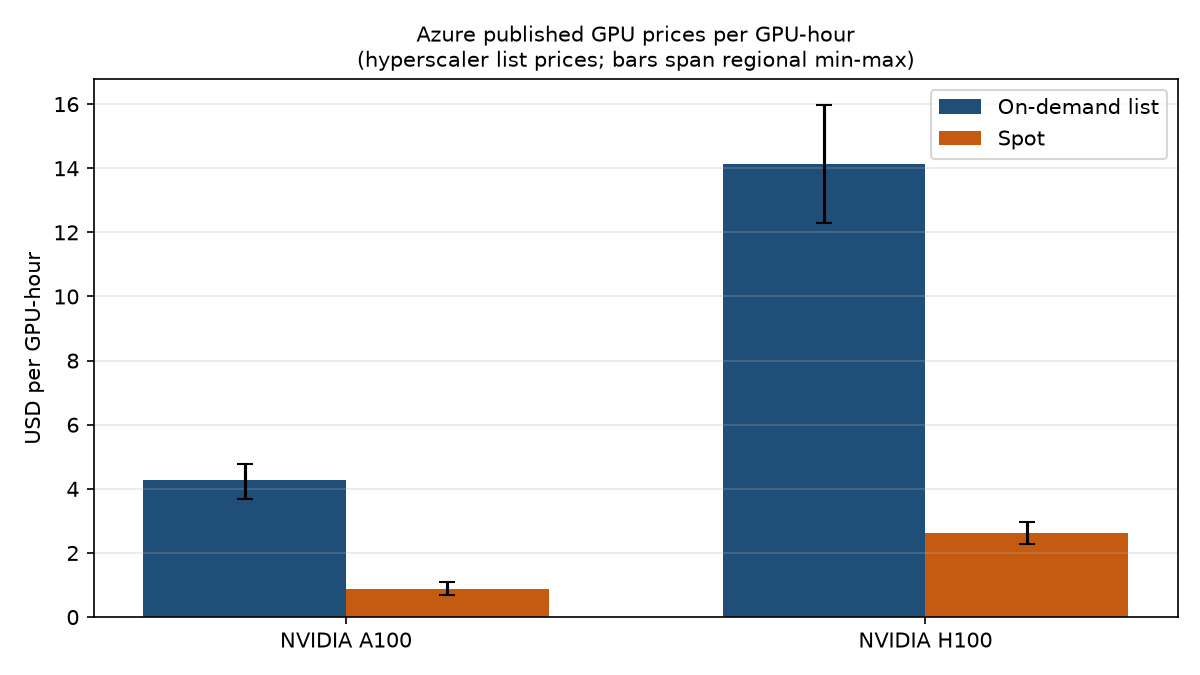
\includegraphics[width=0.85\textwidth]{../figures/compute_price_per_gpu_hour.png}
  \caption{Published Azure GPU prices per GPU-hour. Bars span the
  regional minimum to maximum. On-demand list price is an upper bound on
  realised revenue; spot is shown for contrast, not as a revenue proxy.}
  \label{fig:compute-price}
\end{figure}

Two observations follow immediately, and both bear on the central thesis.

First, \textbf{the dispersion within the compute price is at least as
large as the dispersion in power costs that motivates this paper}. Spot
prices for the same H100 silicon clear roughly a fifth of the on-demand
list price. A merit order computed against ``the'' compute price is
therefore underdetermined until one says \emph{which} compute price;
Section~\ref{sec:merit-order} must present a band, not a line.

Second, \textbf{the hyperscaler on-demand list price is not the price
that disciplines the marginal operator}. Published neocloud index levels
sit near the hyperscaler \emph{spot} price rather than its list price,
which suggests the marginal capacity-clearing price is closer to the
former. We flag this as a hypothesis to test rather than a result: our
own basket currently contains only hyperscaler SKUs, and a neocloud leg
is required before the comparison can be made within one consistent
methodology (see Section~\ref{sec:limitations}).

\subsection{The power cost leg}

\todopending{per-hub power price tables and figures --- the DE-LU
pipeline is implemented and tested but requires an API token that was not
available; no values have been pulled}.

\section{The merit order}
\label{sec:merit-order}

The central deliverable of this project is a merit-order curve: all
tracked capacity sorted ascending by marginal cost per GPU-hour, against
which a reader can compare a compute-price line to see what capacity is
uneconomic at that price. \todopending{this figure requires shutdown
prices for multiple hubs and is not yet computable from a single
pipeline; see \texttt{models/} backlog}.

\section{Constraint analysis: chips vs.\ power}
\label{sec:constraints}

\todopending{interconnection-queue and grid-headroom data collection is
Phase 2 of this project and has not started as of this draft; see open
GitHub issues}.

\section{Sensitivity}
\label{sec:sensitivity}

We commit in advance to varying delivered\_kW, non-power opex, PUE, and
compute price, and reporting where the two central claims
(Section~\ref{sec:intro}) break down rather than merely where they hold.
\todopending{sensitivity tables once Section~\ref{sec:spread}'s inputs
are populated with real data}.

\section{Limitations}
\label{sec:limitations}

This draft is intentionally incomplete, and we list every gap rather than
smooth over it:
\begin{itemize}
  \item \textbf{No pulled data yet.} The ENTSO-E DE-LU pipeline
    (\texttt{pipelines/entsoe.py}) is implemented and tested against a
    synthetic fixture, but has not been run against the live API: it
    requires a free \texttt{ENTSOE\_API\_TOKEN} that was not available in
    the environment this draft was produced in. See
    \texttt{docs/SOURCES.md} for registration steps.
  \item \textbf{Ten of twelve hubs are not started.} Only DE-LU has a
    pipeline; the remaining European zones, US ISOs, Singapore, and the
    document-derived hubs (Gulf states, China, India) are tracked as
    GitHub issues, not estimated.
  \item \textbf{GPU counts per site are not disclosed} by operators in
    general, so installed/announced capacity figures will rely on
    third-party estimates (CBRE, DC Byte) with their own uncertainty.
  \item \textbf{PUE is self-reported} by operators where published at
    all, and the \SI{1.25}{} figure used as this project's default is an
    industry-typical value, not a measurement.
  \item \textbf{PPA (power purchase agreement) prices are confidential}
    in most jurisdictions; this project uses public wholesale/day-ahead
    prices as a proxy, which will differ from actual contracted rates,
    typically understating the compute operator's true cost certainty
    (and sometimes its price level) in either direction depending on
    contract structure.
  \item \textbf{Gulf and China data, when added, will be
    document-derived} (government/TSO reports, not live APIs), and will
    carry \texttt{confidence=low} accordingly.
  \item \textbf{The compute-price leg is the weakest input, and the
    asymmetry is structural.} A survey conducted 2026-08-03
    (\texttt{docs/SOURCES.md}) found no free, redistributable
    compute-price index of comparable quality to the power data. The two
    credible indices identified --- Silicon Data's \texttt{SDH100RT} and
    GetDeploying's GPU rental price index --- are both paywalled, and the
    latter's terms explicitly prohibit redistributing raw data feeds,
    which is incompatible with publishing a CC-BY-4.0 dataset. This
    project therefore adopts a free-sources-only constraint and rejects
    both, constructing its own index from vendor-published list prices
    instead (Section~\ref{sec:regional}). We take the weaker source and
    say so rather than compromise reproducibility, but the reader should
    note that our compute-price series is consequently narrower than the
    commercial indices it replaces.
  \item \textbf{The compute-price basket is currently one vendor and one
    segment.} It contains Azure SKUs only, so it measures hyperscaler
    list pricing rather than the market. AWS and GCP publish free price
    lists and belong in the cohort; more importantly, no neocloud
    provider is represented yet, which means the segment dispersion this
    paper argues is central cannot yet be measured within a single
    consistent methodology. Every dispersion figure we report is
    therefore a lower bound.
  \item \textbf{On-demand list price is not the realised price.} Large
    operators transact on multi-year reserved contracts at material and
    confidential discounts. This is the exact mirror of the PPA problem
    on the power side: \emph{both} legs of the spread are public proxies
    for confidential real transactions.
  \item \textbf{Ordering and level have different confidence.} Which hub
    goes uneconomic first depends mainly on the power leg and is
    comparatively robust; the absolute compute price at which it happens
    depends on the weak leg. We hedge these two claims differently
    throughout, and readers should not transfer confidence from the
    former to the latter.
\end{itemize}

\section{Conclusion}
\label{sec:conclusion}

\todopending{to be written once Section~\ref{sec:merit-order} and
Section~\ref{sec:constraints} have real results to conclude from. This
project is under active, multi-session construction; see the GitHub
repository's Issues and Milestones for current status rather than a
prose summary here, per the project's own contribution rules.}

\bibliographystyle{plainnat}
\bibliography{references}

\end{document}
